
\section{Compiler's Effect on the Code}

\begin{frame}[fragile]{Example C++ Code}
\begin{block}{}
    Quicksort implementation with Lomuto's partition scheme.
\end{block}
\begin{lstlisting}[language=C++]
void quicksort( int low, int high){

    int i;
    if(low < high ){
        i = partition( low, high);
            quicksort( low, i - 1);
            quicksort( i + 1, high);
    }
}
\end{lstlisting}   
\end{frame}
\begin{frame}[fragile]{Example C++ Code}
\begin{lstlisting}[language=C++]
    int partition (int low, int high){
    int i = low;
    int j = low;
    float Pivot = sort.getValue(high); 
    while (sort.getValue(i) <= Pivot && sort.getValue(j) <= Pivot && j < high -1){
        j++;
        i++;
    }
    while ( j < high){
        j++;
        if(sort.getValue(j) < Pivot)
            sort.swap(i,j);
        while(sort.getValue(i) <= Pivot && i < j)
            i++;
    }
    if(j == high)
        sort.swap(i, high);
    return i;
}
\end{lstlisting}
\end{frame}


\begin{frame}{Compiler Optimisations}
    
\begin{figure}
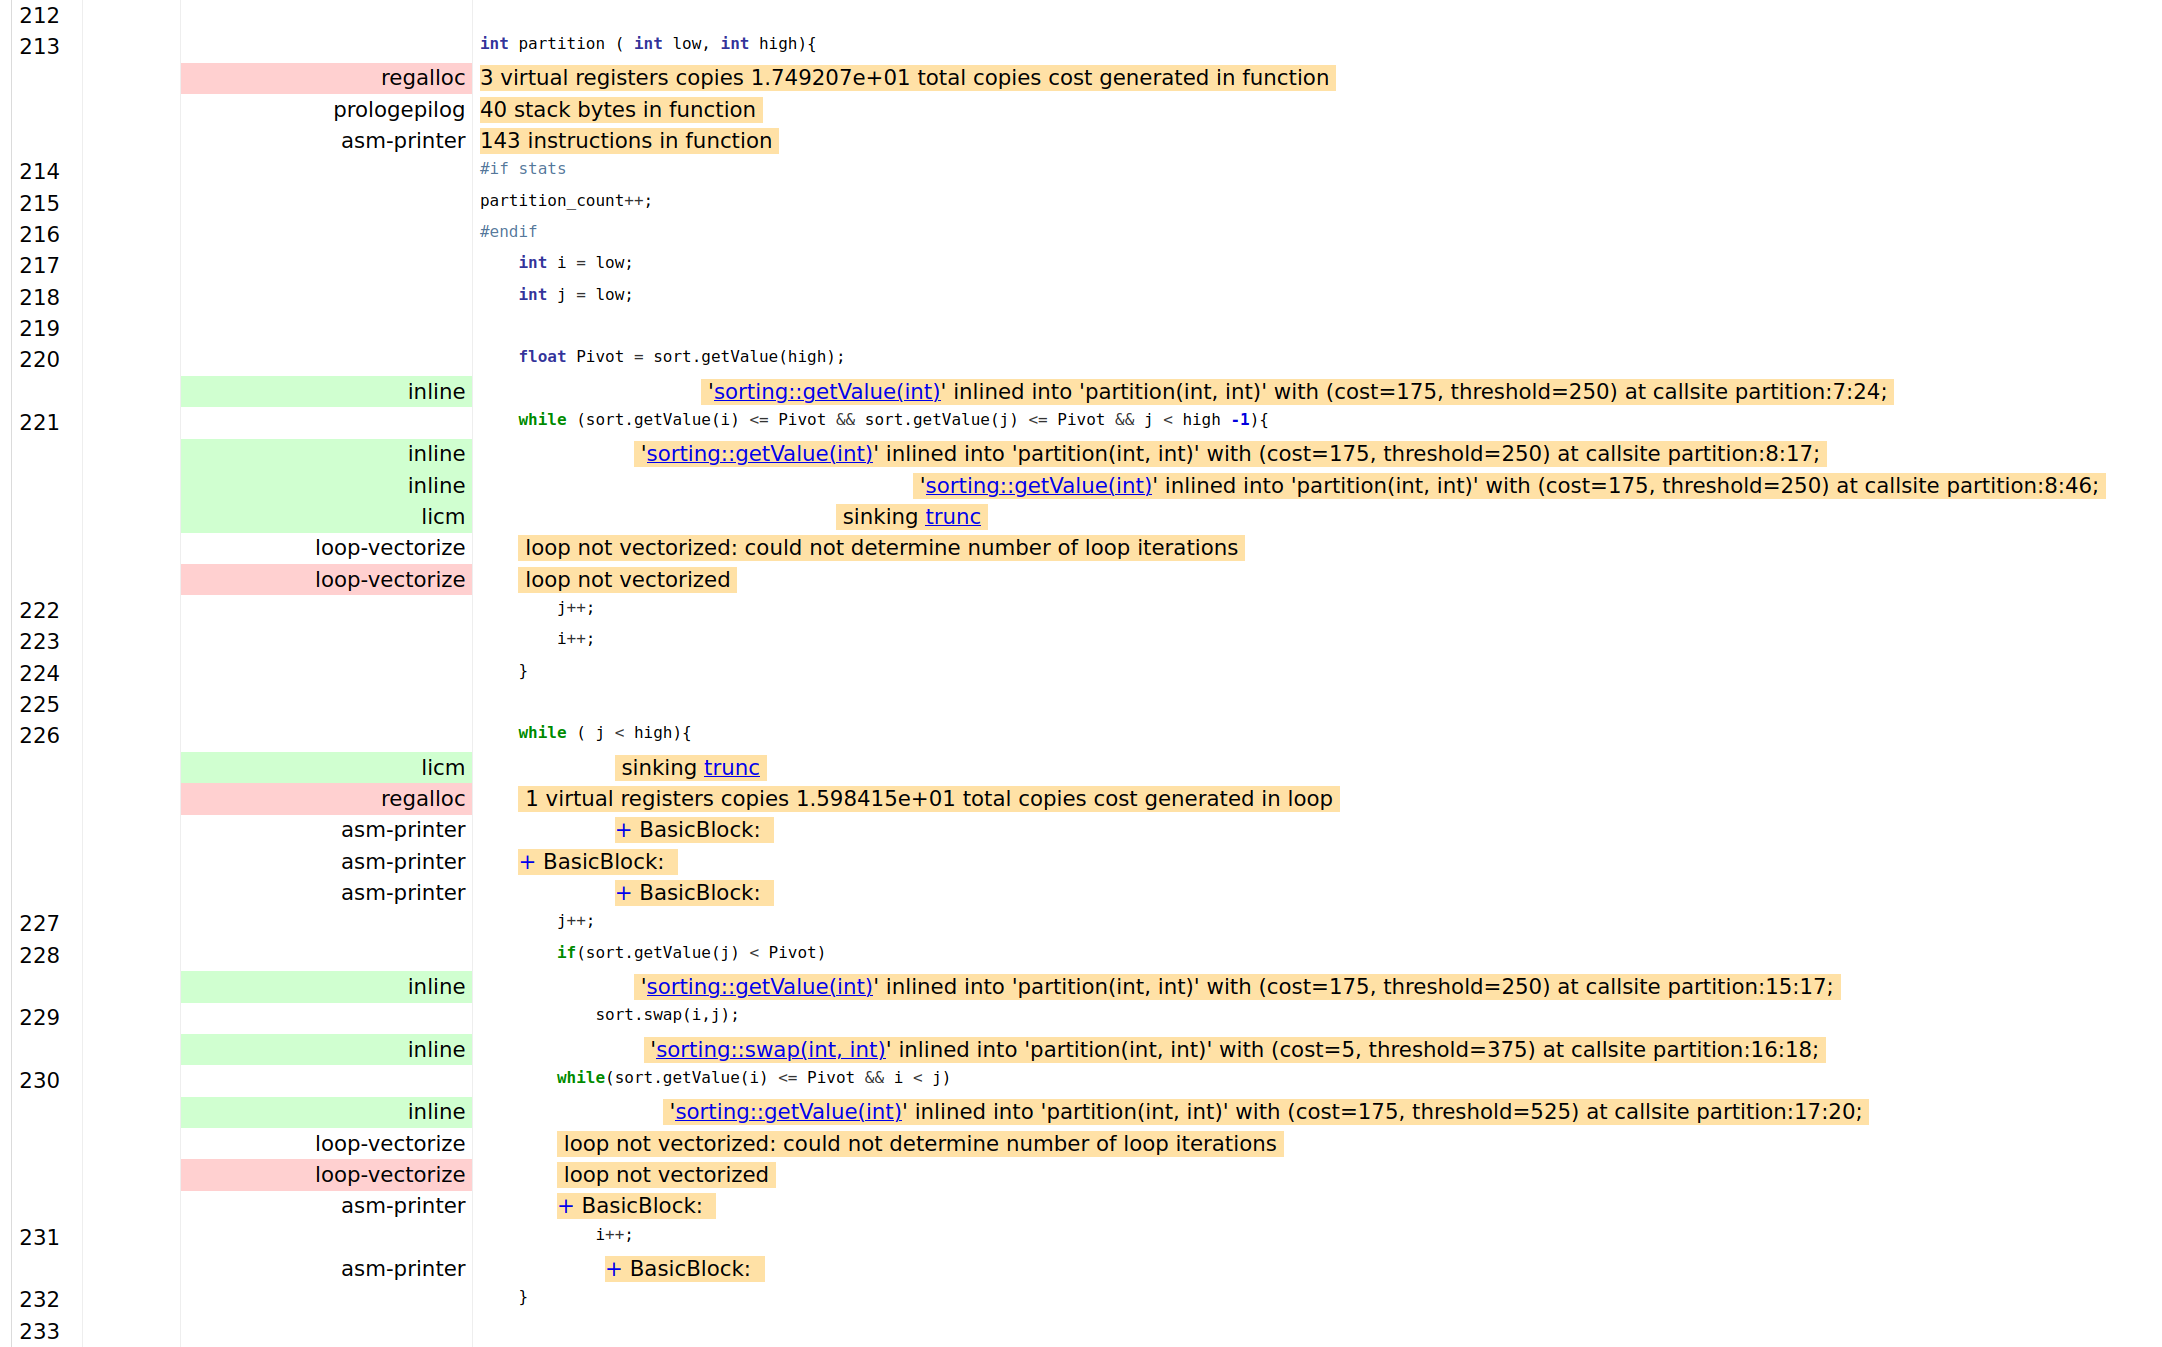
\includegraphics[width=0.8\textwidth]{partition_optviewer.png}
\caption{Optimisations of Clang provided by Opt-Viewer}
\label{part_opt}
\end{figure}
\end{frame}

\begin{frame}{Compiler Optimisations}
    
\begin{figure}
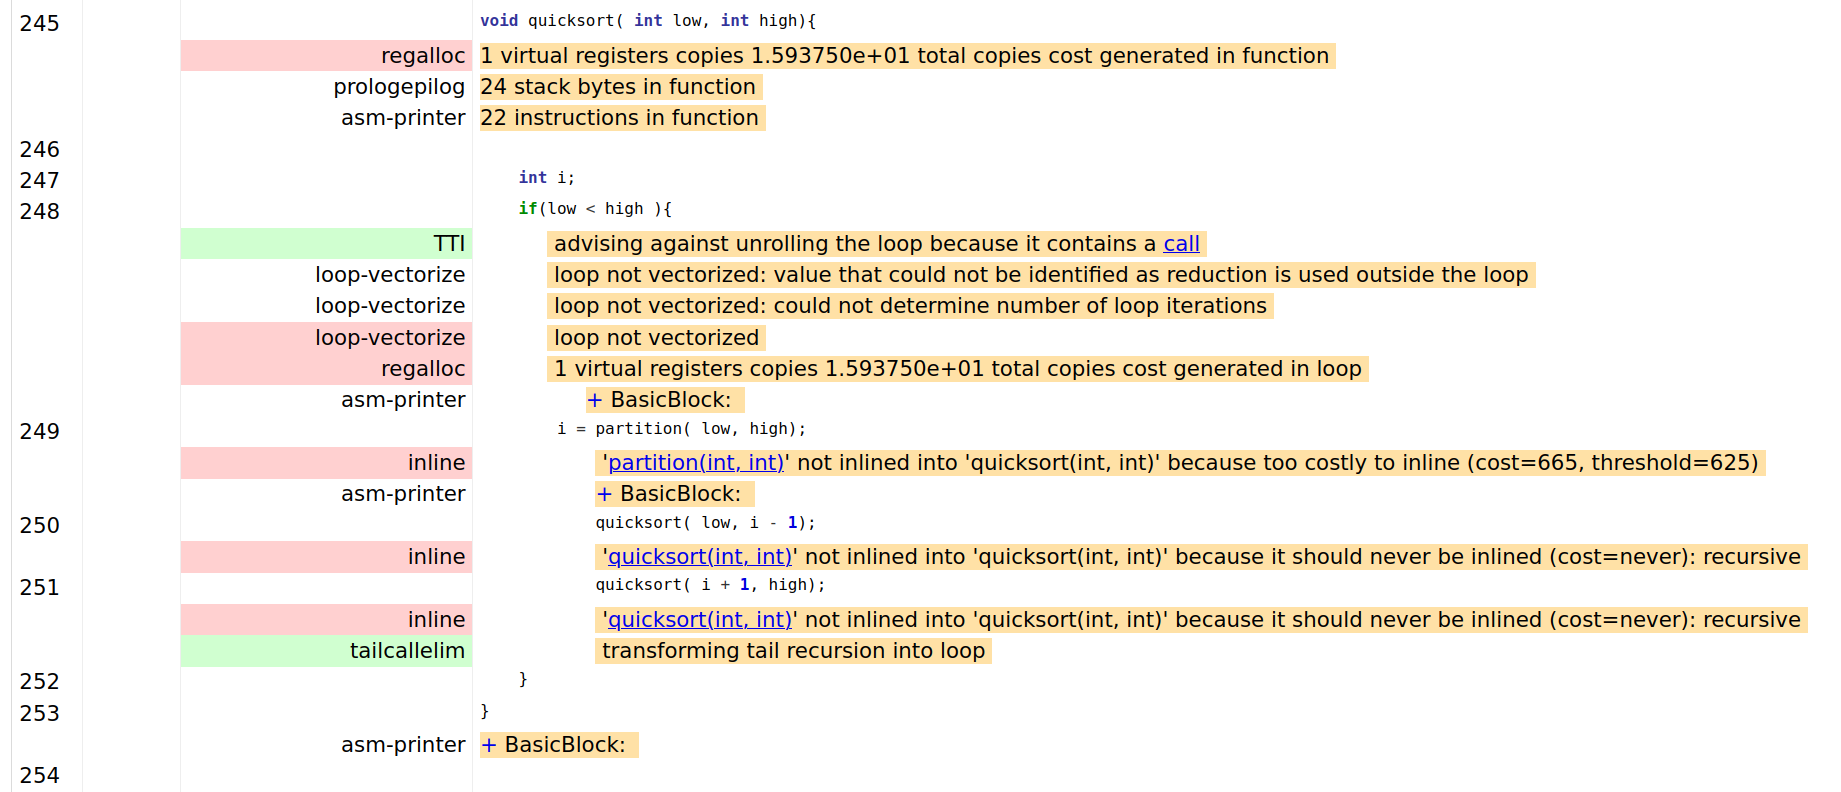
\includegraphics[width=0.8\textwidth]{quicksort_optviewer.png}
\caption{Optimisations of Clang provided by Opt-Viewer}
\label{qs_opt}
\end{figure}
\end{frame}
